% ======================================================================
% Preámbulo y estilo — "Huellas del universo"
% Base: tema metropolis + paleta ITeDA de la defensa de tesis y de RAFA 2026.
% Compilar con LuaLaTeX (ver compilar.sh).
% ======================================================================
\usetheme[progressbar=frametitle, sectionpage=none, numbering=fraction,
          block=fill]{metropolis}

\usepackage[spanish,es-noshorthands,es-nodecimaldot,es-tabla]{babel}
\usepackage{fontspec}
\usepackage{unicode-math}
\setsansfont{Fira Sans}[
  UprightFont = *-Book, BoldFont = *-SemiBold,
  ItalicFont = *-BookItalic, BoldItalicFont = *-SemiBoldItalic]
\setmainfont{Fira Sans}[
  UprightFont = *-Book, BoldFont = *-SemiBold,
  ItalicFont = *-BookItalic, BoldItalicFont = *-SemiBoldItalic]
\setmathfont{Fira Math}
\setmonofont{Fira Mono}

\usepackage{graphicx}
\usepackage{booktabs}
\usepackage{array}
\usepackage{xparse}
\usepackage{siunitx}
\sisetup{output-decimal-marker={,}, exponent-product=\times,
         group-separator={.}, group-minimum-digits=5}
\usepackage{tikz}
\usetikzlibrary{arrows.meta, positioning, calc, decorations.pathmorphing,
  decorations.markings, decorations.pathreplacing, shapes.geometric,
  shadows.blur, backgrounds, fadings, patterns}
\usepackage{pgfplots}
\pgfplotsset{compat=1.18}
\usepgfplotslibrary{fillbetween}
\usepackage[most]{tcolorbox}
\usepackage{appendixnumberbeamer}
\usepackage{fontawesome5}

\graphicspath{{figures/}}

% ----------------------------------------------------------------------
% Paleta ITeDA (la misma de la defensa) + colores auxiliares
% ----------------------------------------------------------------------
\definecolor{itedaTeal}{HTML}{1B5E7E}
\definecolor{itedaTealDark}{HTML}{123847}
\definecolor{itedaOrange}{HTML}{F07E26}
\definecolor{itedaLight}{HTML}{F5F7F8}
\definecolor{itedaGray}{HTML}{5A6B72}
\definecolor{noche}{HTML}{0B1E27}
\definecolor{hielo}{HTML}{7FD3F0}
\definecolor{cmbRojo}{HTML}{C0392B}
\definecolor{cmbAzul}{HTML}{2C6FB7}
\definecolor{verdeRadio}{HTML}{2E8B57}
\definecolor{violetaNu}{HTML}{7B4FB5}

\setbeamercolor{palette primary}{bg=itedaTeal, fg=white}
\setbeamercolor{palette secondary}{bg=itedaTealDark, fg=white}
\setbeamercolor{palette tertiary}{bg=itedaTealDark, fg=white}
\setbeamercolor{frametitle}{bg=itedaTeal, fg=white}
\setbeamercolor{title separator}{fg=itedaOrange}
\setbeamercolor{progress bar}{fg=itedaOrange, bg=itedaTeal!35}
\setbeamercolor{progress bar in head/foot}{fg=itedaOrange, bg=itedaTeal!35}
\setbeamercolor{normal text}{fg=itedaTealDark}
\setbeamercolor{alerted text}{fg=itedaOrange}
\setbeamercolor{example text}{fg=itedaTeal}
\setbeamercolor{background canvas}{bg=white}
\setbeamercolor{itemize item}{fg=itedaOrange}
\setbeamercolor{itemize subitem}{fg=itedaTeal}
\setbeamercolor{block title}{bg=itedaTeal, fg=white}
\setbeamercolor{block body}{bg=itedaLight, fg=itedaTealDark}
\setbeamercolor{frame numbering}{fg=itedaGray}

\setbeamertemplate{navigation symbols}{}
\setbeamerfont{frametitle}{size=\large, series=\bfseries}
\setbeamerfont{footnote}{size=\tiny}
\setbeamerfont{itemize/enumerate body}{size=\small}
\setbeamerfont{itemize/enumerate subbody}{size=\small}
\setlength{\leftmargini}{1.1em}

% ----------------------------------------------------------------------
% Etiqueta del bloque narrativo, a la derecha de la barra de título.
% Reemplaza a las portadas de sección.
% ----------------------------------------------------------------------
\def\bloqueactual{}
\newcommand{\bloque}[1]{\gdef\bloqueactual{#1}}
\addtobeamertemplate{frametitle}{}{%
  \ifx\bloqueactual\empty\else
  \begin{tikzpicture}[remember picture, overlay]
    \node[anchor=north east, xshift=-0.25cm, yshift=-0.26cm,
          font=\scriptsize\bfseries, text=white, fill=itedaTealDark,
          rounded corners=1.5pt, inner sep=2.6pt]
      at (current page.north east) {\bloqueactual};
  \end{tikzpicture}\fi}

% ----------------------------------------------------------------------
% Fondos a sangre completa.  \fondo[oscurecer][w|h]{archivo}
%   w: la imagen ocupa el ancho (se recorta arriba/abajo)
%   h: la imagen ocupa el alto  (se recorta a los costados)
% ----------------------------------------------------------------------
\NewDocumentCommand{\fondo}{O{0} O{w} m}{%
  \begin{tikzpicture}[remember picture, overlay]
    \begin{scope}
      \clip (current page.south west) rectangle (current page.north east);
      \if#2w
        \node[inner sep=0pt] at (current page.center)
          {\includegraphics[width=\paperwidth]{#3}};
      \else
        \node[inner sep=0pt] at (current page.center)
          {\includegraphics[height=\paperheight]{#3}};
      \fi
      \fill[black, opacity=#1] (current page.south west) rectangle
        (current page.north east);
    \end{scope}
  \end{tikzpicture}}

% Degradado oscuro desde un borde, para que el texto se lea sobre fotos.
\NewDocumentCommand{\velo}{O{0.75} m}{%
  \begin{tikzpicture}[remember picture, overlay]
    \ifx#2l
      \shade[left color=black, right color=black, opacity=#1,
        path fading=east] (current page.south west) rectangle
        ([xshift=0.62\paperwidth]current page.north west);
    \fi
    \ifx#2b
      \shade[bottom color=black, top color=black, opacity=#1,
        path fading=north] (current page.south west) rectangle
        ([yshift=0.45\paperheight]current page.south east);
    \fi
    \ifx#2t
      \shade[bottom color=black, top color=black, opacity=#1,
        path fading=south] ([yshift=-0.35\paperheight]current page.north west)
        rectangle (current page.north east);
    \fi
  \end{tikzpicture}}

% Créditos discretos (abajo a la derecha). \credito{...}  /  \creditoblanco{...}
% (en frames con número de página, se corre a la izquierda para no pisarlo)
\newcommand{\credito}[1]{%
  \begin{tikzpicture}[remember picture, overlay]
    \node[anchor=south east, xshift=-1.45cm, yshift=0.12cm,
      font=\fontsize{5.5}{6.5}\selectfont, text=itedaGray, align=right]
      at (current page.south east) {#1};
  \end{tikzpicture}}
\newcommand{\creditoblanco}[1]{%
  \begin{tikzpicture}[remember picture, overlay]
    \node[anchor=south east, xshift=-0.18cm, yshift=0.12cm,
      font=\fontsize{5.5}{6.5}\selectfont, text=white!75, align=right]
      at (current page.south east) {#1};
  \end{tikzpicture}}
% Variante abajo a la izquierda (para no pisar el número de página)
\newcommand{\creditoizq}[1]{%
  \begin{tikzpicture}[remember picture, overlay]
    \node[anchor=south west, xshift=0.18cm, yshift=0.12cm,
      font=\fontsize{5.5}{6.5}\selectfont, text=itedaGray, align=left]
      at (current page.south west) {#1};
  \end{tikzpicture}}

% Insignia para marcar ilustraciones esquemáticas o resultados preliminares
\newcommand{\insignia}[2][itedaGray]{%
  {\setlength{\fboxsep}{1.6pt}\colorbox{#1}{%
   \textcolor{white}{\fontsize{6.5}{7}\selectfont\bfseries\MakeUppercase{#2}}}}}
\newcommand{\esquematico}{\insignia{ilustración esquemática}}
\newcommand{\preliminar}{\insignia[itedaOrange]{preliminar}}

% Pregunta destacada
\newcommand{\pregunta}[1]{{\color{itedaOrange}\bfseries #1}}

% Caja para ecuaciones o ideas clave
\newtcolorbox{clave}[1][]{colback=itedaLight, colframe=itedaTeal,
  boxrule=0pt, leftrule=2.2pt, arc=0pt, left=4pt, right=4pt, top=3pt,
  bottom=3pt, fontupper=\small, before upper={\raggedright}, #1}
\newtcolorbox{claveoscura}[1][]{colback=black!55, colframe=itedaOrange,
  opacityback=0.85, boxrule=0pt, leftrule=2.2pt, arc=0pt, left=5pt, right=5pt,
  top=3pt, bottom=3pt, fontupper=\small\color{white}, before upper={\raggedright}, #1}

% Número grande + leyenda (para "cifras que importan")
\newcommand{\cifra}[2]{%
  \begin{minipage}[t]{\linewidth}\centering
    {\fontsize{19}{21}\selectfont\bfseries\color{itedaOrange}#1}\\[1pt]
    {\footnotesize #2}
  \end{minipage}}

% ----------------------------------------------------------------------
% Mapa de Argentina: \geo{lon}{lat} -> coordenadas TikZ dentro de un
% \mapa de ancho \mapW y alto \mapH (extensión igual a mapa_argentina.py).
% ----------------------------------------------------------------------
\newlength{\mapH}\newlength{\mapW}
\newcommand{\geo}[2]{({(#1+76)/24*\mapW},{(#2+56)/36*\mapH})}
\newcommand{\mapabase}[1]{%  #1 = alto
  \setlength{\mapH}{#1}\setlength{\mapW}{0.52528\mapH}%
  \node[anchor=south west, inner sep=0pt] at (0,0)
    {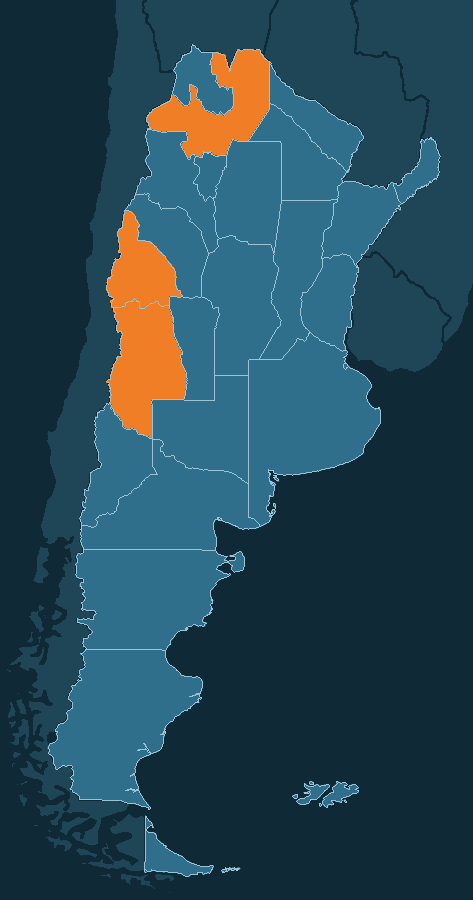
\includegraphics[height=\mapH]{generadas/mapa_argentina.pdf}};}

% Mapa de Sudamérica (scripts/mapa_sudamerica.py): lon -82..-32, lat -56..6
\newlength{\mapSAH}\newlength{\mapSAW}
\newcommand{\geoSA}[2]{({(#1+82)/50*\mapSAW},{(#2+56)/62*\mapSAH})}
\newcommand{\mapaSA}[1]{%
  \setlength{\mapSAH}{#1}\setlength{\mapSAW}{0.73089\mapSAH}%
  \node[anchor=south west, inner sep=0pt] at (0,0)
    {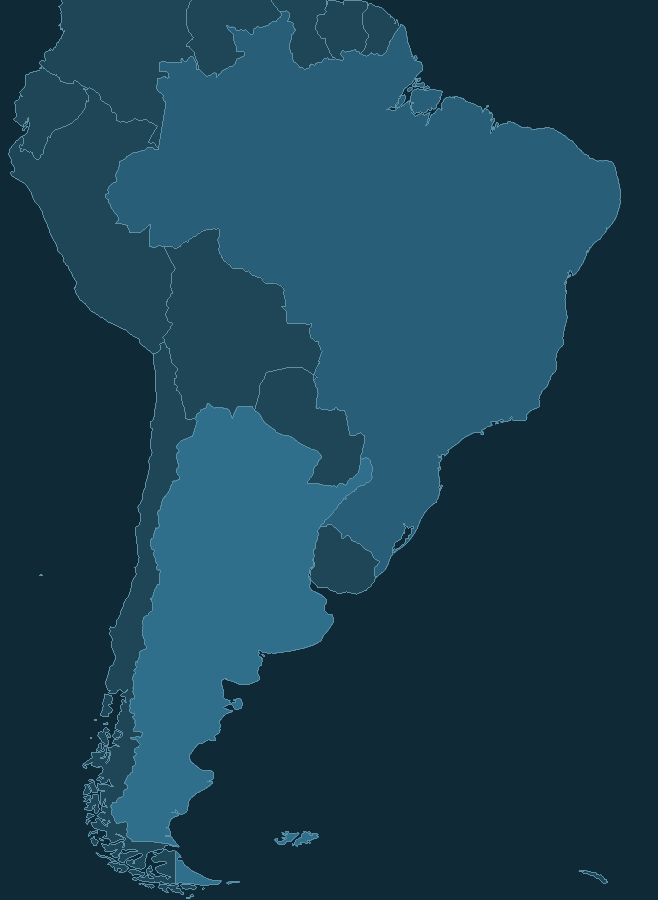
\includegraphics[height=\mapSAH]{generadas/mapa_sudamerica.pdf}};}

% Estilos de PGFPlots coherentes con la paleta
\pgfplotsset{
  coloquio/.style={
    axis line style={itedaGray}, tick style={itedaGray},
    every tick label/.append style={font=\scriptsize, text=itedaTealDark},
    label style={font=\footnotesize, text=itedaTealDark},
    legend style={font=\scriptsize, draw=none, fill=white, fill opacity=0.85,
      text opacity=1},
    /pgf/number format/use comma, /pgf/number format/1000 sep={},
    clip mode=individual,
    grid style={itedaGray!18}, major grid style={itedaGray!18},
  }}

% Flechas y nodos frecuentes
\tikzset{
  flecha/.style={-{Stealth[length=2.2mm]}, thick},
  foton/.style={decorate, decoration={snake, amplitude=0.6mm,
    segment length=2mm, post length=1.5mm}, -{Stealth[length=1.8mm]}},
  etiqueta/.style={font=\footnotesize, text=itedaTealDark},
}
